\begin{center}
    \fbox{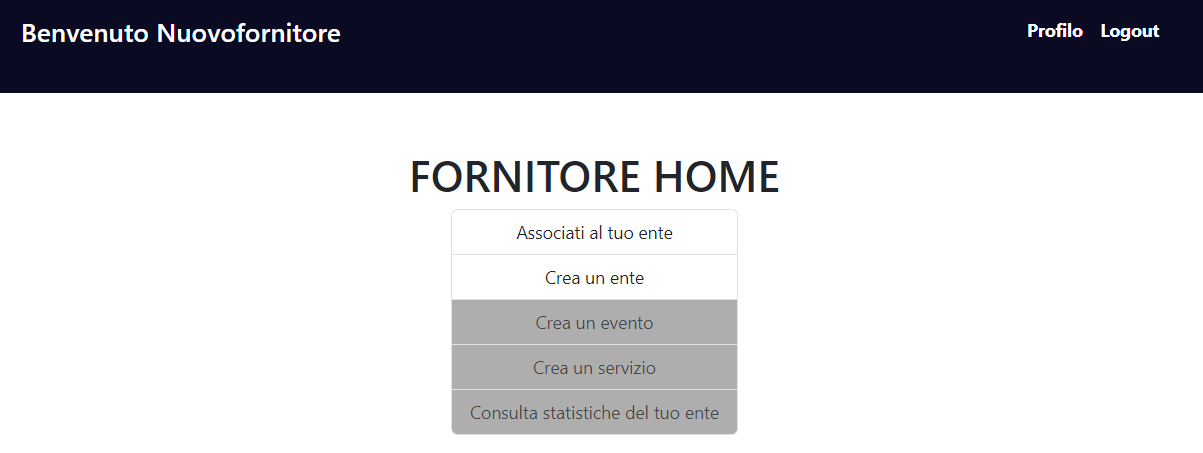
\includegraphics[width=0.95\columnwidth]{fornitore_home_1.png}}
\end{center}
Una volta effettuato il primo accesso come fornitore l'applicativo offre le seguenti possibilità:
\begin{itemize}
    \item Associarsi ad un ente
    \item Creare un ente
\end{itemize}
\begin{center}
    \fbox{
\includegraphics[width=0.95\columnwidth]{fornitore_home_2.png}}
\end{center}
Il tasto "Associa al tuo ente" permette al fornitore di potersi associare ad un ente già registrato all'interno della piattaforma mente il tasto "Crea un ente" permette di creare da zero un ente con il quale associarsi. Le altre funzionalità rimarranno disabilitate fino a che non verrà associato un ente.
\begin{itemize}
    \item Creare un evento
    \item Creare un servizio
    \item Consultazione delle statistiche degli eventi, del saldo e dei servizi
\end{itemize}
\begin{center}
    \fbox{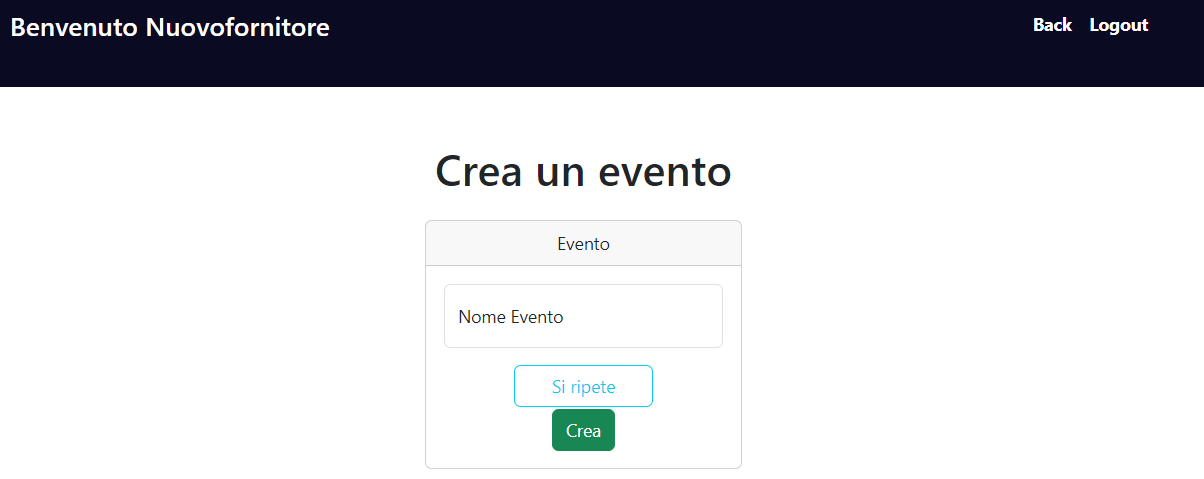
\includegraphics[width=0.95\columnwidth]{fornitore_evento.png}}
\end{center}
\begin{center}
    \fbox{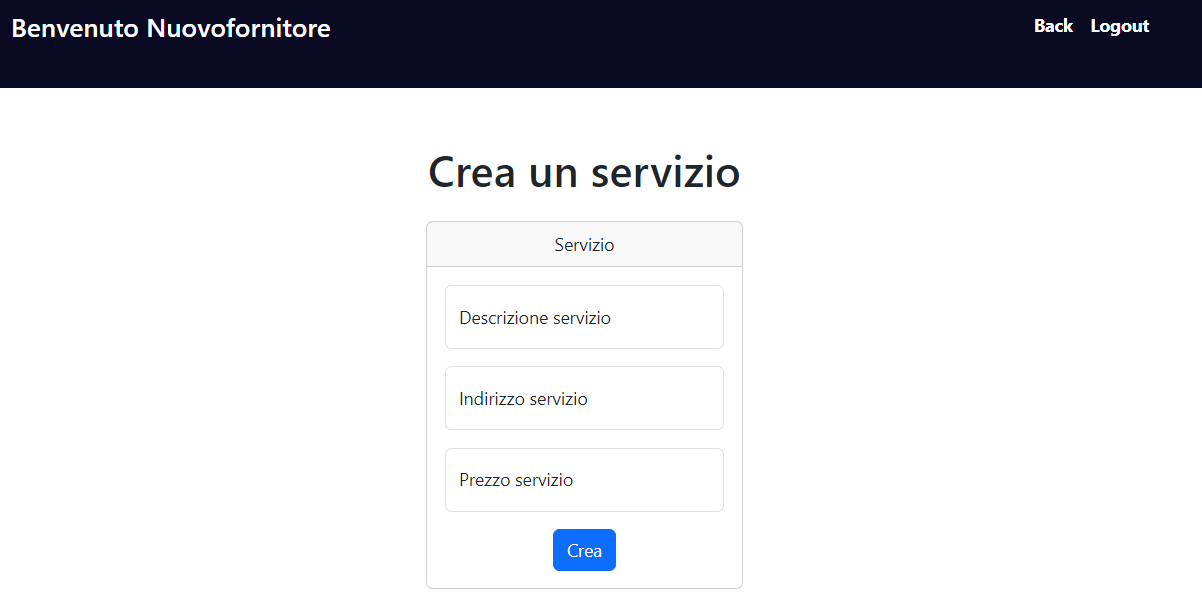
\includegraphics[width=0.95\columnwidth]{fornitore_servizio.png}}
\end{center}
I successivi comandi permettono di creare un evento (sia occasionale che periodico con gli appositi tasti) oppure un servizio.
\begin{center}
    \fbox{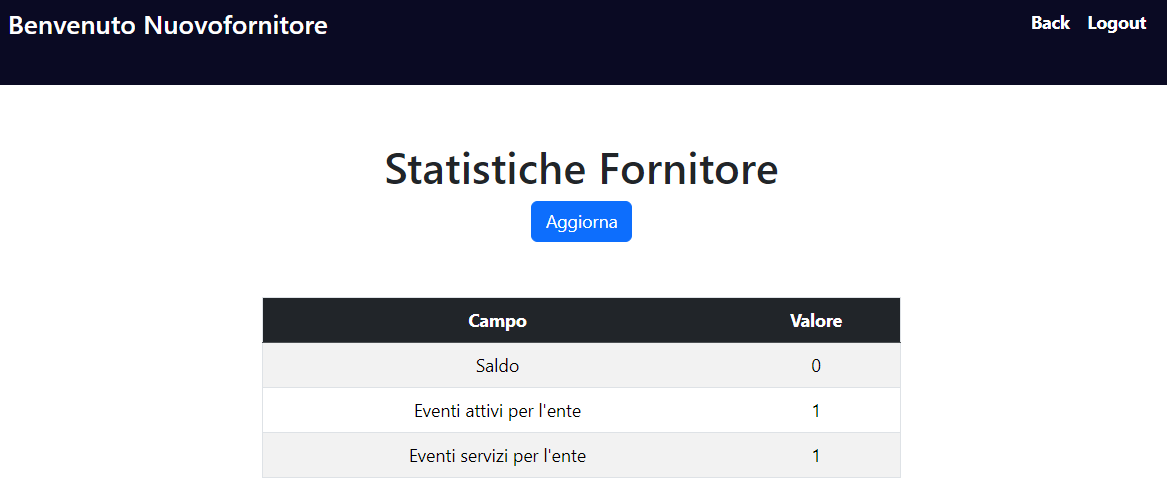
\includegraphics[width=0.95\columnwidth]{fornitore_statistiche.png}}
\end{center}
La consultazione delle statistiche saldo e servizi permettono rispettivamente di consultare il saldo accumulato dalla registrazione di eventi e dall'acquisto di servizi.



